\chapter{نرم ‌افزار و ارتباطات}


\section{ارتباطات و سرور}

\subsection{اتصال بیسیم دوربین به سرور}

%در این بخش از پایان‌نامه، به توضیح نحوه اتصال ماژول ESP32 CAM به روتر از طریق کد آردوینو و همچنین توضیح نوشتن یک مدیر دستگاه برای سرور در فایل apphttpd.cpp می‌پردازیم.% 
\subsubsection{مفاهیم اصلی}
در این بخش به تبیین مفاهیمی از شبکه
\noindent\unskip\LTRfootnote{Network}
که مورد استفاده قرار گرفته اند و تشریح فرآیندهای انجام شده برای برقراری ارتباط بین ماژول
\lr{ESP32 CAM} 
و سرور پرداخته شده‌است. در شبکه‌های اینترنتی دو مفهوم پرکاربرد با کلیدواژه نقطه دسترسی
\noindent\unskip\LTRfootnote{Access Point}
و مُد
\noindent\unskip\LTRfootnote{Mode}
ایستگاهی
\noindent\unskip\LTRfootnote{Station}
(یا به اختصار
\lr{STA})
وجود دارد. 
طبق تعریف، نقطه دسترسی
\cite{AccessPoint}
یک دستگاه سخت افزاری شبکه‌است که به سایر دستگاه ها اجازه می‌دهد به یک شبکه سیمی متصل شوند و به عنوان یک دستگاه مستقل، ممکن است یک اتصال سیمی به یک روتر
\noindent\unskip\LTRfootnote{Router}
داشته باشد. اگرچه در یک روتر بی سیم، می تواند جزء جدایی ناپذیر خود روتر نیز باشد.


احتمالا تجربه متصل کردن تلفن همراه و یا سایر وسایل الکترونیکی خود به مودم خانگی را داشته اید. در این حالت تلفن همراه در مُد ایستگاهی جهت دریافت آی پی
\noindent\unskip\LTRfootnote{Internet Protocol address}
از مودم و همچنین مودم نیز در حالت نقطه دسترسی قرار گرفته‌است. به همین طریق ماژول
\lr{ESP32-CAM}
نیز به عنوان یک دستگاه الکترونیکی و به دلیل نوع طراحی و قابلیت ارتباط بیسیم، می‌تواند به مودم و حتی تلفن همراه در حالت نقطه دسترسی متصل گردد. 
\begin{figure}[H]
	\centering
	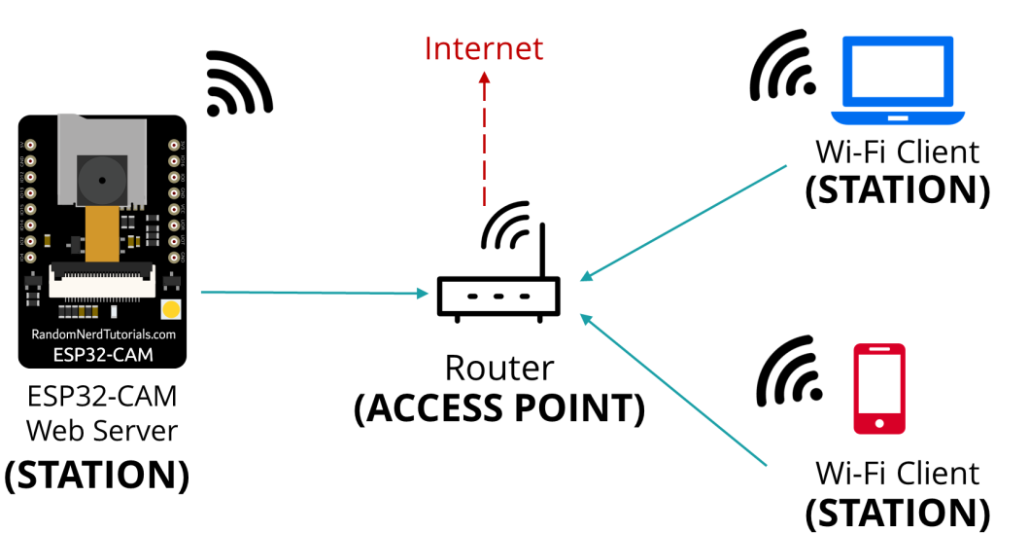
\includegraphics[width=0.5\textwidth]{./images/Chapter3/RouterAsAccessPoint}	
	\caption[نقطه دسترسی و مُد ایستگاهی]{نحوه ارتباط اجزای شبکه \cite{Network}}
	\label{}
\end{figure}
\noindent
\unskip

\subsubsection{شبه‌کد و تشریح جزئیات برنامه}
در ادامه، به‌طور دقیق‌تر، فرآیند اتصال ماژول به مودم با استفاده از برنامه نوشته شده در محیط آردوینو را تشریح خواهیم کرد. سپس نحوه استفاده از کتابخانه‌های ارتباط بیسیم برای اتصال به شبکه و اخذ آدرس پروتکل اینترنت \lr{(IP)} به‌عنوان یک مشخصه‌ی مهم برای دستگاه خواهد آمد.
%در اینجا، تعریف و پیاده‌سازی یک مسیر (Route) در فایل apphttpd.cpp برای دریافت درخواست‌های ارسالی از دستگاه تصویربردار انجام می‌پذیرد. سپس توضیح مراحل پردازش درخواست و ارسال پاسخ به دستگاه از طریق این مسیر را ارائه خواهیم داد.%

\section*{}
\begin{latin}
	\lstinputlisting[style=python_style]{code/Pseudocodes/NetworkPseudocode.py}
\end{latin}
در ابتدا به نحوه تنظیم پارامترهای شبکه اعم از نام شبکه \lr{(SSID)} و رمز عبور \lr{(Password)} اشاره می‌کنیم. 
نخست باید مدل دوربین با توجه به ماژول مورد استفاده در برنامه تعریف می‌شود. در این بین دوربین \lr{OV2640} در دسته \lr{AI THINKER} قرار می‌گیرد. سپس نام شبکه و رمزعبور مودم مورد استفاده را در برنامه قرار داده و به تنظیم پارامتر های مهمی در بخش \lr{Setup} در محیط آردوینو پرداخته می‌شود.

%\begin{figure}[h]
%	\centering
%	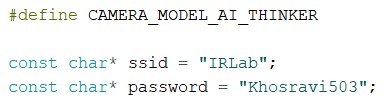
\includegraphics[width=0.3\textwidth]{./images/Chapter3/SSIDPass}	
%	\caption{}
%	\label{}
%\end{figure}
نخست مشخصه \lr{Buad rate} را که بیانگر تعداد تغییرات در سطح سیگنال در یک ثانیه است، برابر 115200 قرار داده شده و سپس پارامترهای تصویر اعم از اندازه تصویر
\noindent\unskip\LTRfootnote{Frame size}،
کیفیت تصویر
\lr{(Jpeg quality)} 
\noindent\unskip\LTRfootnote{Jpeg quality}
و... تنظیم گردید. 

\section*{}
\begin{latin}
	\lstinputlisting[style = cplus_style]{code/CameraWebServer/CameraWebServer.ino}
\end{latin}

در ادامه پیکربندی تعیین شده برای دوربین بررسی گردیده و در صورت عدم وجود خطا در پیکربندی اتصال به روتر شروع می‌گردد. همانطور که در قطعه کد زیر مشخص است با قرار دادن دستورات چاپ در خطوط مختلف برنامه از اتصال کامل ماژول به روتر اطمینان حاصل می‌گردد.
\section*{}
\begin{latin}
	\lstinputlisting[style = cplus_style]{code/CameraWebServer/CameraBegin.ino}
\end{latin}


درانتها نیز آدرس محلی
\noindent\unskip\LTRfootnote{LocalIP}
که روتر به ماژول اختصال می‌دهد، در بخش سریال مانیتور
\noindent\unskip\LTRfootnote{Serial Monitor}
آردوینو چاپ می‌گردد. نتیجه این اتصال در شکل س قابل مشاهده است.
\newpage
\subsection{سرور و هندلر‌‌ها }
\subsubsection{نحوه کارکرد سرور و نقش هندلر‌ها}
در سامانه‌های وب، ارتباط و تبادل اطلاعات بین دستگاه‌ها و سرور
\noindent\unskip\LTRfootnote{Server}
از طریق ارسال درخواست‌
\noindent\unskip\LTRfootnote{Request}
و دریافت پاسخ‌
\noindent\unskip\LTRfootnote{Respond}
به‌وسیله پروتکل های \lr{HTTP} و \lr{HTTPS} و...‌صورت می‌گیرد. وقتی که یک دستگاه یا مرورگر اینترنتی درخواستی به سرور ارسال می‌کند، این درخواست اطلاعاتی از قبیل نوع عملیات  (\lr{DELETE} ،\lr{PUT} ، \lr{POST} ، \lr{GET} و...) و آدرس مورد نظر(\lr{URL})
\noindent\unskip\LTRfootnote{Uniform Resource Locator}
را شامل می‌شود. سرور در این زمان تجزیه و تحلیل درخواست را انجام می‌دهد و با توجه به محتوا و ماهیت درخواست، یک منطق مناسب را فعال می‌سازد.این عملیات‌ها ممکن است شامل دسترسی به پایگاه داده، پردازش اطلاعات، تولید پاسخ‌های مناسب و دیگر عملیات باشند.

در اینجا نقش هندلر
\noindent\unskip\LTRfootnote{Handler}
ها به عنوان یکی از اجزای اصلی سیستم به چشم می‌خورد.هندلرها مسئول پردازش درخواست‌ها و انجام عملیات‌های مختلف میان سرور و دستگاه‌ها هستند. هندلرها اطلاعات درخواست را تجزیه و تحلیل می‌کنند و بر اساس آن‌ها عملیات‌های مورد نیاز را انجام می‌دهند. به عبارت دیگر می‌توان گفت که هندلرها، ارتباط بین دستگاه‌ها و سرور را به صورت منظم و سازماندهی شده‌ای صورت داده و در نتیجه به بهبود عملکرد و کارایی سامانه کمک می‌کند. 

\subsubsection{شبه‌کد و تشریح جزئیات برنامه }
در زیر شبه‌کد
\noindent\unskip\LTRfootnote{Pseudo code}
این بخش مختصرا قراره داده شده و پس از آن به تشریح کامل‌تر آن پرداخته خواهد شد.

\section*{}
\begin{latin}
	\lstinputlisting[style=python_style]{code/Pseudocodes/HandlerPseudocode.py}
\end{latin}

در قطعه برنامه زیر چند هندلر برای مُد‌های مختلف احتمالی تعریف شده‌است. برخی از آنها برای ماژول
\lr{ESP32-CAM}
از پیش تعریف شده‌اند. مهمترین هندلری که با هدف ارسال و مانیتورینگ اطلاعات بین سرور و ماژول و به طبع آن برد
\lr{STM32}
پیاده‌سازی شد،
\lr{current\_color\_uri}
نام دارد. برای این هندلر مقدار
\lr{uri}
که بیانگر مسیر
\noindent\unskip\LTRfootnote{Path}
در آدرس است،
\lr{/currentColor}
تعریف شد. تابع هندلر آن در ادامه بطور کامل‌تر تعریف شده است.
هدف از تعریف این هندلر
\label{PurposeOfOurHandler}
آن است که درخواست ارسال شده به سرور که حاوی اطلاعاتی اعم از رنگ مانع تشخیص داده شده توسط ربات، فاصله ربات تا مانع و... است را دریافت کرده و این اطلاعات از طریق ارتباط
\lr{USART}
, بصورت برخط و با کمترین تاخیر به برد
\lr{STM32}
فرستاده شود.



\section*{}
\begin{latin}
	\lstinputlisting[style = cplus_style]{code/CameraWebServer/defineHandlers.cpp}
\end{latin}

در ادامه چند کانفیگ برای دوربین تنظیم شده که به دلیل طولانی بودن در بخش زیر ذکر نشده‌اند. سپس با بررسی یک شرط، در صورت ارسال موفقیت‌آمیز درخواست از طرف سیستم، تمامی هندلر‌ها چک می‌شوند تا در صورت نیاز پاسخ مناسب را به آن درخواست برگردانند.

\section*{}
\begin{latin}
	\lstinputlisting[style = cplus_style]{code/CameraWebServer/HTTPRequestSendOrNot.cpp}
\end{latin}

همانطور که ذکر شد
\ref{PurposeOfOurHandler}
می‌بایست هندلر مورد نظر طوری تعریف شود تا اطلاعات مدنظر به بهترین شکل مدیریت شود.
به همین جهت برای ارسال اطلاعات از کوئری استرینگ
\noindent\unskip\LTRfootnote{Query String}
استفاده شده‌است.

\subsubsection{کوئری استرینگ}

‏گاهی‌اوقات لازم است که وب‌سایت از وضعیت
\noindent\unskip\LTRfootnote{State}
ما مطلع باشد و بتواند در همان لحظه، مسیری را طی کند. مثلا زمانی که قصد داریم یک فرم چند صفحه‌ای را پر کنیم، سرور باید مطلع باشد که ما در صفحه پیش چه کاری انجام دادیم و یا به عنوان مثالی دیگر می‌توان به مراحل یک خرید اینترنتی (اضافه کردن کالاها به سبد خرید، پرداخت آنلاین و...) اشاره کرد.

پروتکل
\lr{HTTP}
امکان نگهداری وضعیت را ندارد. پس مکانیزم‌های دیگری به‌وجود آمدند تا بتوانند این کار را انجام دهند. از جمله‌ی این مکانیزم‌ها می‌توان به نگهداری وضعیت سمت سرور با استفاده از 
\lr{Session}
و یا نگهداری وضعیت سمت کاربر
\noindent\unskip\LTRfootnote{Client}
با استفاده از کوکی
\noindent\unskip\LTRfootnote{Cookie}
اشاره کرد.
مکانیزم دیگری برای نگهداری وضعیت و انتقال اطلاعات بين صفحات وجود دارد. در این مکانیزم همراه با درخواست‌ها، وضعیت قبلی را نیز از طریق
\lr{URL}
جدیدی که فراخوانی می‌شود، به سرور داده می‌شود. به این روش کوئری استرینگ گفته می‌شود.
\newpage
کوئری استرینگ هر مقداریست که بعد از علامت سوال $(“?”)$ در انتهای
\lr{URL}
قرار می‌گیرد که می‌تواند یک یا تعداد بیشتری پارامتر باشد.

ساختار کوئری استرینگ را در شکل زیر مشاهده می‌کنید:
\begin{figure}[H]
	\centering
	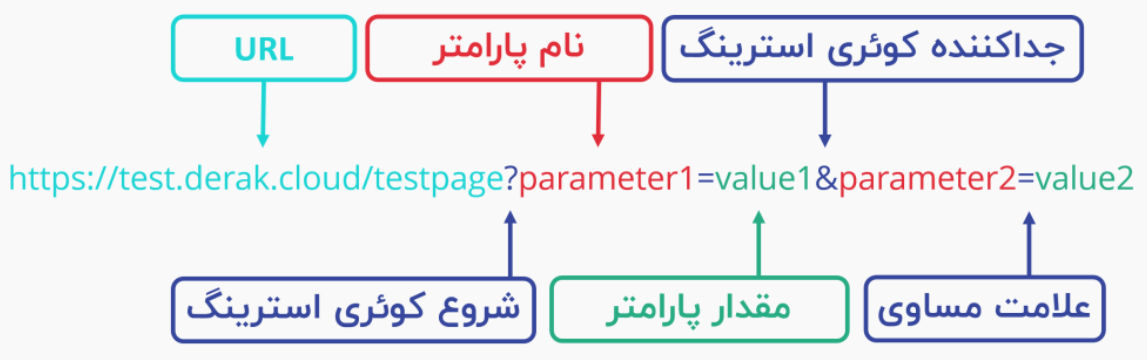
\includegraphics[width=0.7\textwidth]{./images/Chapter3/QueryStringStructure}	
	\caption[ساختار کوئری استرینگ]{ساختار کوئری استرینگ \cite{QueryString}}
	\label{ساختار کوئری}
\end{figure}
\noindent
\unskip

همانطور که در شکل
\ref{ساختار کوئری}
مشخص است آدرس های شامل کوئری استرینگ دارای بخش‌های مختلفی می‌باشند.
\begin{itemize}
	\item 
	\lr{URL} : این بخش شامل دامنه مورد نظر است. همچنین از اجزای دیگر آن می‌توان به پروتکل، زیردامنه و مسیر اشاره کرد که در نهایت یک آدرس را تشکیل می‌دهد.
	\item
	$?$ : ابتدای کوئری استرینگ با این علامت شروع می‌شود و پس از آدرس قرار می‌گیرد.
	\item
	نام پارامتر: در کوئری استرینگ پارامترهای مختلف را می‌بینیم که هر پارامتر یک نام
	\noindent\unskip\LTRfootnote{Key}
	و یک مقدار
	\noindent\unskip\LTRfootnote{Value}
	دارد. پس از علامت سوال، نام اولین پارامتر دیده می‌شود.
	\item
	$=$ : برای تعیین مقدار یک پارامتر از این علامت استفاده می‌شود و پس از نام پارامتر قرار می‌گیرد.
	\item
	\lr{\&} : برای جداسازی پارامتر‌های مختلف از این علامت استفاده می‌شود. این علامت بین مقدار پارامتر قبلی و نام پارامتر بعدی قرار می‌گیرد.
\end{itemize}
\newpage
استفاده از این روش مزایا و معایب متفاوتی دارد که در ذیل مختصرا به آن‌ها اشاره شده‌است.
\cite{QueryString}
مزایا:
\begin{itemize}
	
	\item
	استفاده ساده
	\item
	سریع‌ترین روش انتقال اطلاعات بين صفحات
	\item
	عدم تحميل عمليات اضافه به سرويس‌دهنده و در نتیجه هزینه‌ی کم
\end{itemize}

معایب:
\begin{itemize}
	
	\item
	اطلاعات، محدود به رشته‌های ساده است (فقط کاراکترهای مجاز)
	\item
	اطلاعات همواره به عنوان يک رشته بازيابی می‌شوند و در صورت نياز باید آن‌ها را به نوع داده مورد نظر تبديل كرد.
	\item
	اطلاعات توسط همه قابل مشاهده‌است. برای مواردی که لازم است اطلاعاتی به‌طور مخفی از يک صفحه به صفحه ديگر ارسال و يا بر روی آن حساسيت خاصی از نظر امنيتی وجود دارد، قابل استفاده نیست.
	\item
	كاربران می توانند محتويات کوئری استرینگ را تغيير داده و در بعضی موارد باعث ایجاد مشکل شوند.
	\item
	تعداد زيادی از مرورگرها برای طول یک
	\lr{URL}
	محدودیت دارند. بنابراين، نمی‌توان حجم بالایی از اطلاعات را در کوئری استرینگ ذخيره كرد.
\end{itemize}

\subsubsection{تابع هندلر}
در زیر شبه‌کد این بخش مختصرا قراره داده شده و پس از آن به تشریح کامل‌تر آن پرداخته خواهد شد.
\section*{}
\begin{latin}
	\lstinputlisting[style=python_style]{code/Pseudocodes/CurrentColorPseudocode.py}
\end{latin}

در برنامه زیر ابتدا یک بافر
\noindent\unskip\LTRfootnote{Buffer}
با مقدار زیاد انتخاب شده و سپس اگر یک درخواست از نوع
\lr{GET}
که دارای کوئری استرینگ باشد برای سرور ارسال شده باشد، آنگاه نام پارامتر آن بررسی می‌شود و اگر برابر
\lr{color}
بوده باشد، مقدار آن پارامتر به عنوان داده معتبر درون بافر ریخته می‌شود. سپس دیتای داخل بافر را از طریق ارتباط
\lr{UART}
برای
\lr{STM32}
ارسال و سپس داده داخل بافر برای درخواست بعدی خالی می‌شود. 
\section*{}
\begin{latin}
	\lstinputlisting[style = cplus_style]{code/CameraWebServer/ColorHandlers.cpp}
\end{latin}

\subsection{ارتباط \lr{USART}}
انتقال اطلاعات را می توان به دو روش کلی موازی و سریال انجام داد.در روش انتقال موازی چند بیت اطلاعات به وسیله چند خط انتقال می‌یابد و در روش انتقال سریال در هر لحظه فقط یک بیت ارسال می‌شود. در مقایسه بین این دو روش می‌توان گفت که در روش انتقال موازی به علت انتقال چند بیت اطلاعات در یک لحظه، سرعت آن نسبت به سریال که در یک لحظه فقط یک بیت را انتقال می‌دهد بیشتر است. همچنین برای فواصل طولانی بکار بردن روش انتقال موازی به علت ازدیاد سیم‌های ارتباطی، دارای هزینه بالا می‌باشد؛ بنابراین در فواصل طولانی انتقال به روش سریال مناسب تر است.

\textbf{فرستنده و گیرنده سریال همزمان و غیر همزمان جهانی} یا \lr{USART } یک ارتباط از نوع انتقال سریال می باشد که امکان ارتباط دوطرفه کامل را می‌دهد و برای ارتباط بین دو دستگاه مفید می‌باشد.
در حالتی که هیچ ارسال و دریافتی انجام نمی‌شود یا اصطلاحاً خط انتقال در حالت بیکار \lr{(Idle)} قرار دارد، سطح ولتاژ مربوط به یک منطقی بر روی خط ارسال قرار می‌گیرد. تغییر وضعیت از یک به صفر منطقی به معنی شروع ارسال است و گیرنده آماده دریافت اطلاعات می‌شود. این صفر شدن به مدت یک بیت باید طول بکشد و به آن "بیت شروع" گفته می‌شود. بعد از آن یک بایت داده به ترتیب از بیت کم ارزش \lr{(LSB)} به بیت پرارزش \lr{(MSB)} ارسال می‌شود. در نهایت یک بیت برای آزمایش شدن درستی داده ارسال شده، روی خط ارسال قرار می‌گیرد که بیت "بیت توازن" نام دارد.

نرخ انتقال‌های که به صورت قراردادی بین فرستنده و گیرنده در یک ارتباط سریال، مشخص می‌شود مقادیر خاصی می‌توانند داشته باشند که مقدارهای ۴۸۰۰، ۱۹۲۰۰ ،۹۶۰۰، ۳۸۴۰۰، ۵۷۶۰۰، ۱۱۵۲۰۰ (بیت بر ثانیه) از معمول‌ترین این مقادیرند. در انجام آزمایش های عملی بر روی ربات از نرخ ۱۱۵۲۰۰ بیت بر ثانیه استفاده شده است.
%مثلاً نرخ انتقال ۹۶۰۰ به این معنی است که در هر ثانیه ۹۶۰۰ بیت منتقل می‌شود. پس هر بیت در فاصلهٔ زمانی ۱۰۴٫۱۶۶ میکروثانیه باید منتقل شود و در تمام این مدت مقدار خود را حفظ کند تا گیرنده نمونه برداری مناسبی انجام دهد.%


\section{اتصال دو برد به یکدیگر}


در این بخش، روش اتصال دو برد \lr{ESP32 CAM } و \lr{STM32f101c8t6} به یکدیگر از طریق رابط \lr{USART} تشریح خواهد شد. رابط \lr{USART} یک رابط سریالی است که امکان انتقال داده‌ها بین دو دستگاه را فراهم می‌کند. این رابط اغلب برای ارتباط میان میکروکنترلرها و ماژول‌ها استفاده می‌شود. استفاده از این روش برای ارتباط بین دو دستگاه از اهمیت ویژه‌ای در تبادل اطلاعات در پروژه‌های الکترونیکی و رباتیک برخوردار است و تجربه کار با رابط‌های سریالی را به ارمغان می‌آورد.

ابتدا به تعیین پایه‌های \lr{RX} و \lr{TX} در هر یک از دو برد پرداخته و تنظیمات مورد نیاز در هر دستگاه برای فعال‌سازی رابط \lr{USART} انجام می‌شود. بدین منظور همانطور که در شکل 
\ref{اتصال دو برد}
مشخص است پایه
\lr{UOR}
از ماژول
\lr{ESP32-CAM}
که برای دریافت اطلاعات تعبیه شده‌است، به پایه
\lr{PA9}
از برد
\lr{STM32}
که برای ارسال اطلاعات تعبیه شده‌است متصل می‌باشد. همچنین پایه
\lr{UOT}
از ماژول
\lr{ESP32-CAM}
که برای ارسال اطلاعات تعبیه شده‌است، به پایه
\lr{PA10}
از برد
\lr{STM32}
که برای دریافت اطلاعات تعبیه شده‌است متصل می‌باشد. برای تامین انرژی مدار نیز پایه زمین هر دو مدار و منبع تغذیه یکسان شده و ولتاژ منبع تغذیه بر روی 5 ولت تنظیم خواهد شد.

\begin{figure}[H]
	\centering
	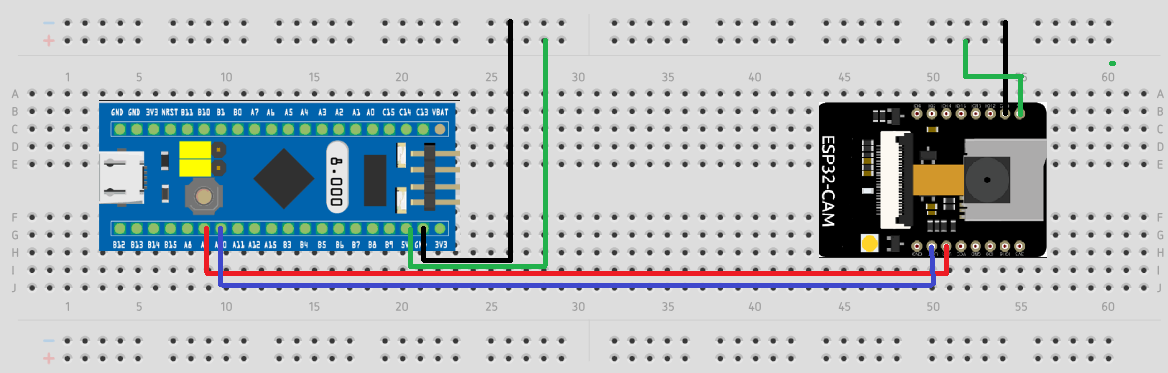
\includegraphics[width=1\textwidth]{./images/Chapter3/TwoBoardConnection}	
	\caption{نحوه اتصال دو برد  به یکدیگر}
	\label{اتصال دو برد}
\end{figure}

\section{جمع‌بندی}


